\documentclass{standalone}
\usepackage{tikz}
\usetikzlibrary{backgrounds, positioning}

\tikzset{
  box/.style  = {draw, rectangle, minimum width=2cm, minimum height=2cm, line width=0.5mm},
  line/.style = {line width=0.5mm},
}

\begin{document}
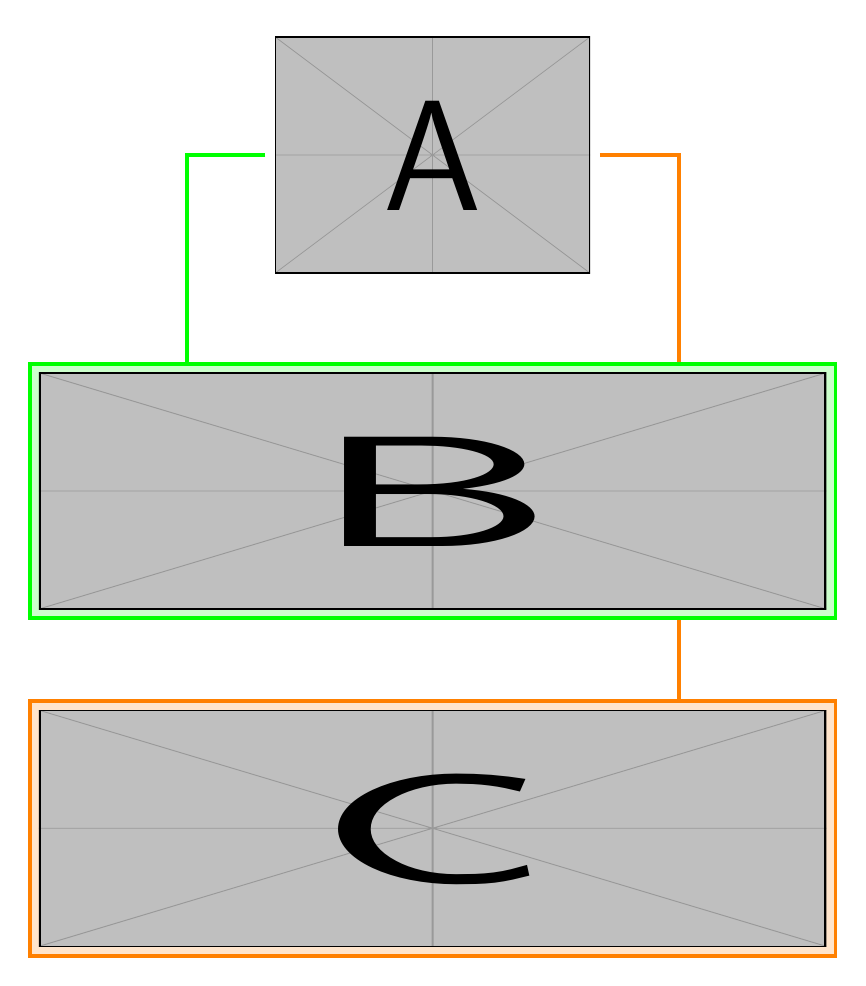
\begin{tikzpicture}[node distance=1cm]
  \node (a) {\includegraphics[width=4cm]{example-image-a}};
  \node (b) [box, draw=green, fill=green!20, below=of a] 
             {\includegraphics[width=10cm,height=3cm]{example-image-b}};
  \node (c) [box, draw=orange, fill=orange!20, below=of b]
             {\includegraphics[width=10cm,height=3cm]{example-image-c}};

  \coordinate[left=of a] (t1);
  \coordinate[right=of a] (t2);

  \draw [line, draw=green] (a) -| (t1 |- b.north);
  \scoped[on background layer]
    \draw [line, draw=orange] (a) -| (t2 |- c.north);
\end{tikzpicture}
\end{document}
